
%(BEGIN_QUESTION)
% Copyright 2009, Tony R. Kuphaldt, released under the Creative Commons Attribution License (v 1.0)
% This means you may do almost anything with this work of mine, so long as you give me proper credit

This Foxboro model 13 DP transmitter is designed to output a pneumatic pressure signal of 3 PSI when there is no process pressure applied to the diaphragm (capsule):

$$\includegraphics[width=15.5cm]{i03938x01.eps}$$

From this information, determine whether the ``zero'' spring is a {\it tension} spring (pulling to the right on the range bar) or a {\it compression} spring (pushing to the left on the range bar).

\vskip 20pt \vbox{\hrule \hbox{\strut \vrule{} {\bf Suggestions for Socratic discussion} \vrule} \hrule}

\begin{itemize}
\item{} Suppose this transmitter output a signal of 3.1 PSI when it should output a signal of 3.0 PSI.  Calculate the error, {\it in percent of span}.
\item{} Suppose this transmitter output a signal of 14.9 PSI when it should output a signal of 15.0 PSI.  Calculate the error, {\it in percent of span}.
\item{} Suppose this transmitter output a signal of 12.4 PSI when it should output a signal of 12.0 PSI.  Calculate the error, {\it in percent of span}.
\item{} Suppose this transmitter output a signal of 8.8 PSI when it should output a signal of 9.0 PSI.  Calculate the error, {\it in percent of span}.
\end{itemize}

\underbar{file i03938}
%(END_QUESTION)





%(BEGIN_ANSWER)

%(END_ANSWER)





%(BEGIN_NOTES)

The Foxboro model 13 transmitter's ``zero'' spring is a {\bf tension} spring, pulling to the right on the bottom of the range bar.  Tension is needed here to give the feedback bellows a force to push against with 3 PSI, since the diaphragm capsule generates no such force for the feedback bellows to react against.






\vfil \eject

\noindent
{\bf Prep Quiz:}

Identify the location of the {\it span} adjustment on this Foxboro model 13A pneumatic pressure transmitter:

$$\includegraphics[width=15.5cm]{i03938x02.eps}$$

\vfil \eject

\noindent
{\bf Prep Quiz:}

Identify the location of the {\it zero} adjustment on this Foxboro model 13A pneumatic pressure transmitter:

$$\includegraphics[width=15.5cm]{i03938x02.eps}$$


%INDEX% Calibration, pneumatic instrument: zero adjustment

%(END_NOTES)


